A continuación, podemos observar dos gráficos que comparan tiempo de ejecución del nuestro algoritmo exacto para grafos creados al azar, utilizando distintos $n$, y para cada $n$, distintos $m$. Para utilizar distintos $m$, consideramos la cantidad de aristas del $K_n$ como la máxima cantidad de aristas posibles, y definimos la cantidad de aristas de cualquier grafo $G$ de $n$ nodos como una proporción con respecto al $K_n$.

\begin{figure}[H]
  \begin{minipage}{0.5\linewidth}
    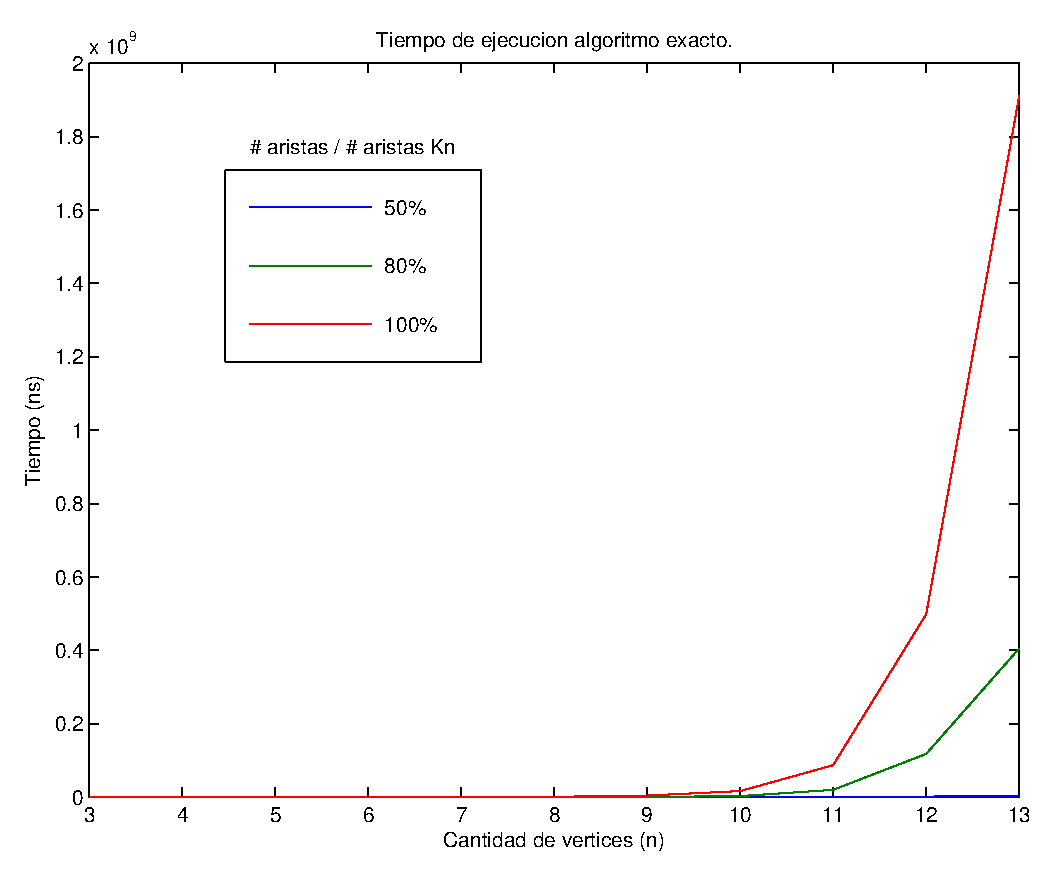
\includegraphics[width=\linewidth]{graficos/exacto_tiempo.eps}
    \caption{Tiempo de ejecución algoritmo exacto}\label{fig:exacto-tiempo}
  \end{minipage}
  \hfill
  \begin{minipage}{0.5\linewidth}
    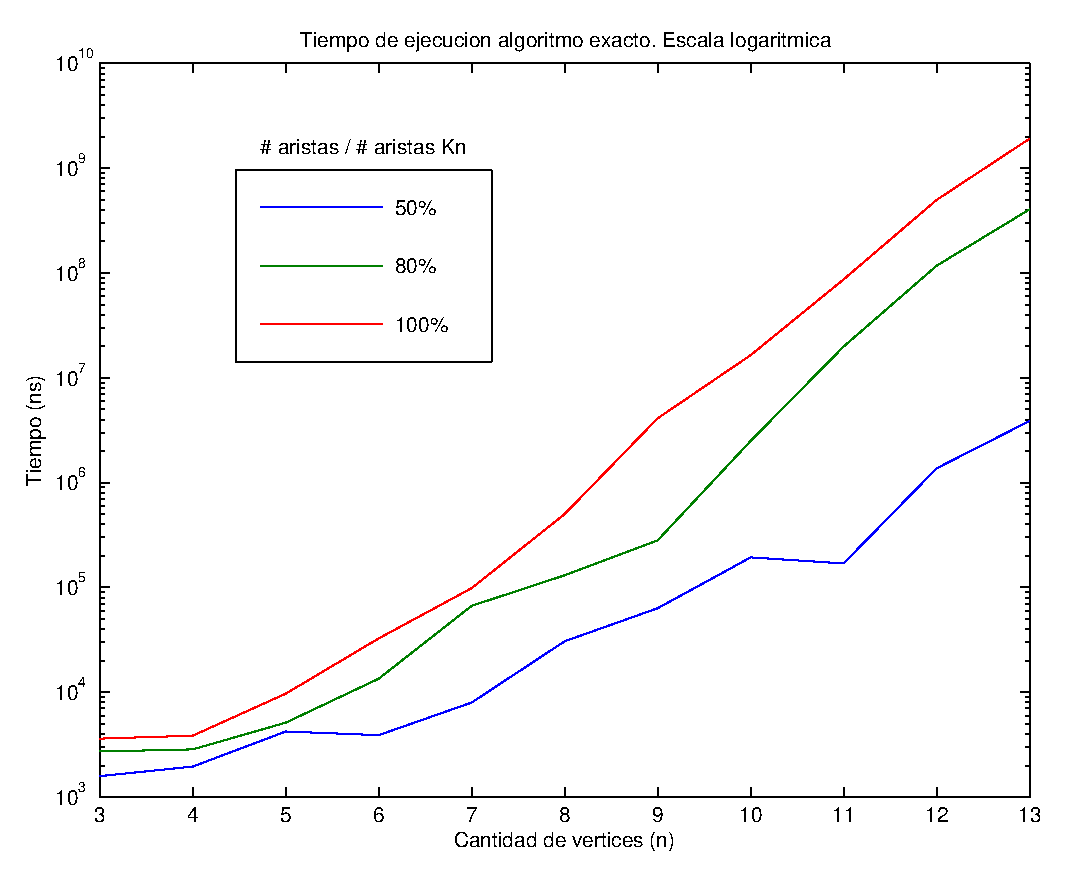
\includegraphics[width=\linewidth]{graficos/exacto_tiempo_log.eps}
    \caption{Idem, escala logarítmica}\label{fig:exacto-tiempo-log}
  \end{minipage}
\end{figure}

Podemos observar empíricamente que nuestro algoritmo exacto se comporta de forma exponencial en los casos medidos. En la figura \ref{fig:exacto-tiempo} no podemos apreciar la relación de tiempo de ejecución entre los distintos grafos. Por esta razón, decidimos incluir otro gráfico con los mismos datos, pero con escala logarítmica para que se pueda apreciar las diferencias entre las distintas corridas.

En la figura \ref{fig:exacto-tiempo-log}, podemos observar que el algoritmo exacto tarda menos cuando tiene menos aristas.	

Por otro lado, como los tiempos de ejecución eran exponenciales incluimos casos hasta $n$ = 13. Con casos con más nodos, el algoritmo exacto tardaba demasiado tiempo en terminar.